\documentclass{article}

\usepackage[%
    left=0.5in,%
    right=0.5in,%
    top=0.5in,%
    bottom=0.5in,%
]{geometry}%
\usepackage{minitoc}
\usepackage{multicol}
\usepackage{graphicx}
\usepackage{fixltx2e}
\usepackage{listings}
\usepackage{color}
\usepackage{hyperref}
    \hypersetup{ colorlinks = true, linkcolor = blue }
\usepackage{blindtext}
\definecolor{lightgray}{gray}{0.9}
\graphicspath{ {./} }

\newcommand{\inlinecode}[2]{\colorbox{lightgray}{\lstinline
[language=#1]$#2$}}
\newcommand{\worddef}[1]{\hyperref[sec:reference]{\textit{#1}}}

\begin{document}

\tableofcontents

\newpage

\section{Architecture}

\begin{multicols}{2}
\begin{itemize}
  \item A software stack for mobile devices
  \item Operating system kernel
  \item Standard middleware
  \begin{itemize}
    \item Android library support
  \end{itemize}
  \item Key applications / user interfaces
  \begin{itemize}
    \item Vendor specific modifications
  \end{itemize}
  \item LK: threading, low level memory management, driver
  \item HAL: libs for hardware module
  \item AR: virtual machine
  \item NCL: fundamental core functionalities
  \item API: programming interface
  \item APP: system apps can be customised.
\end{itemize}

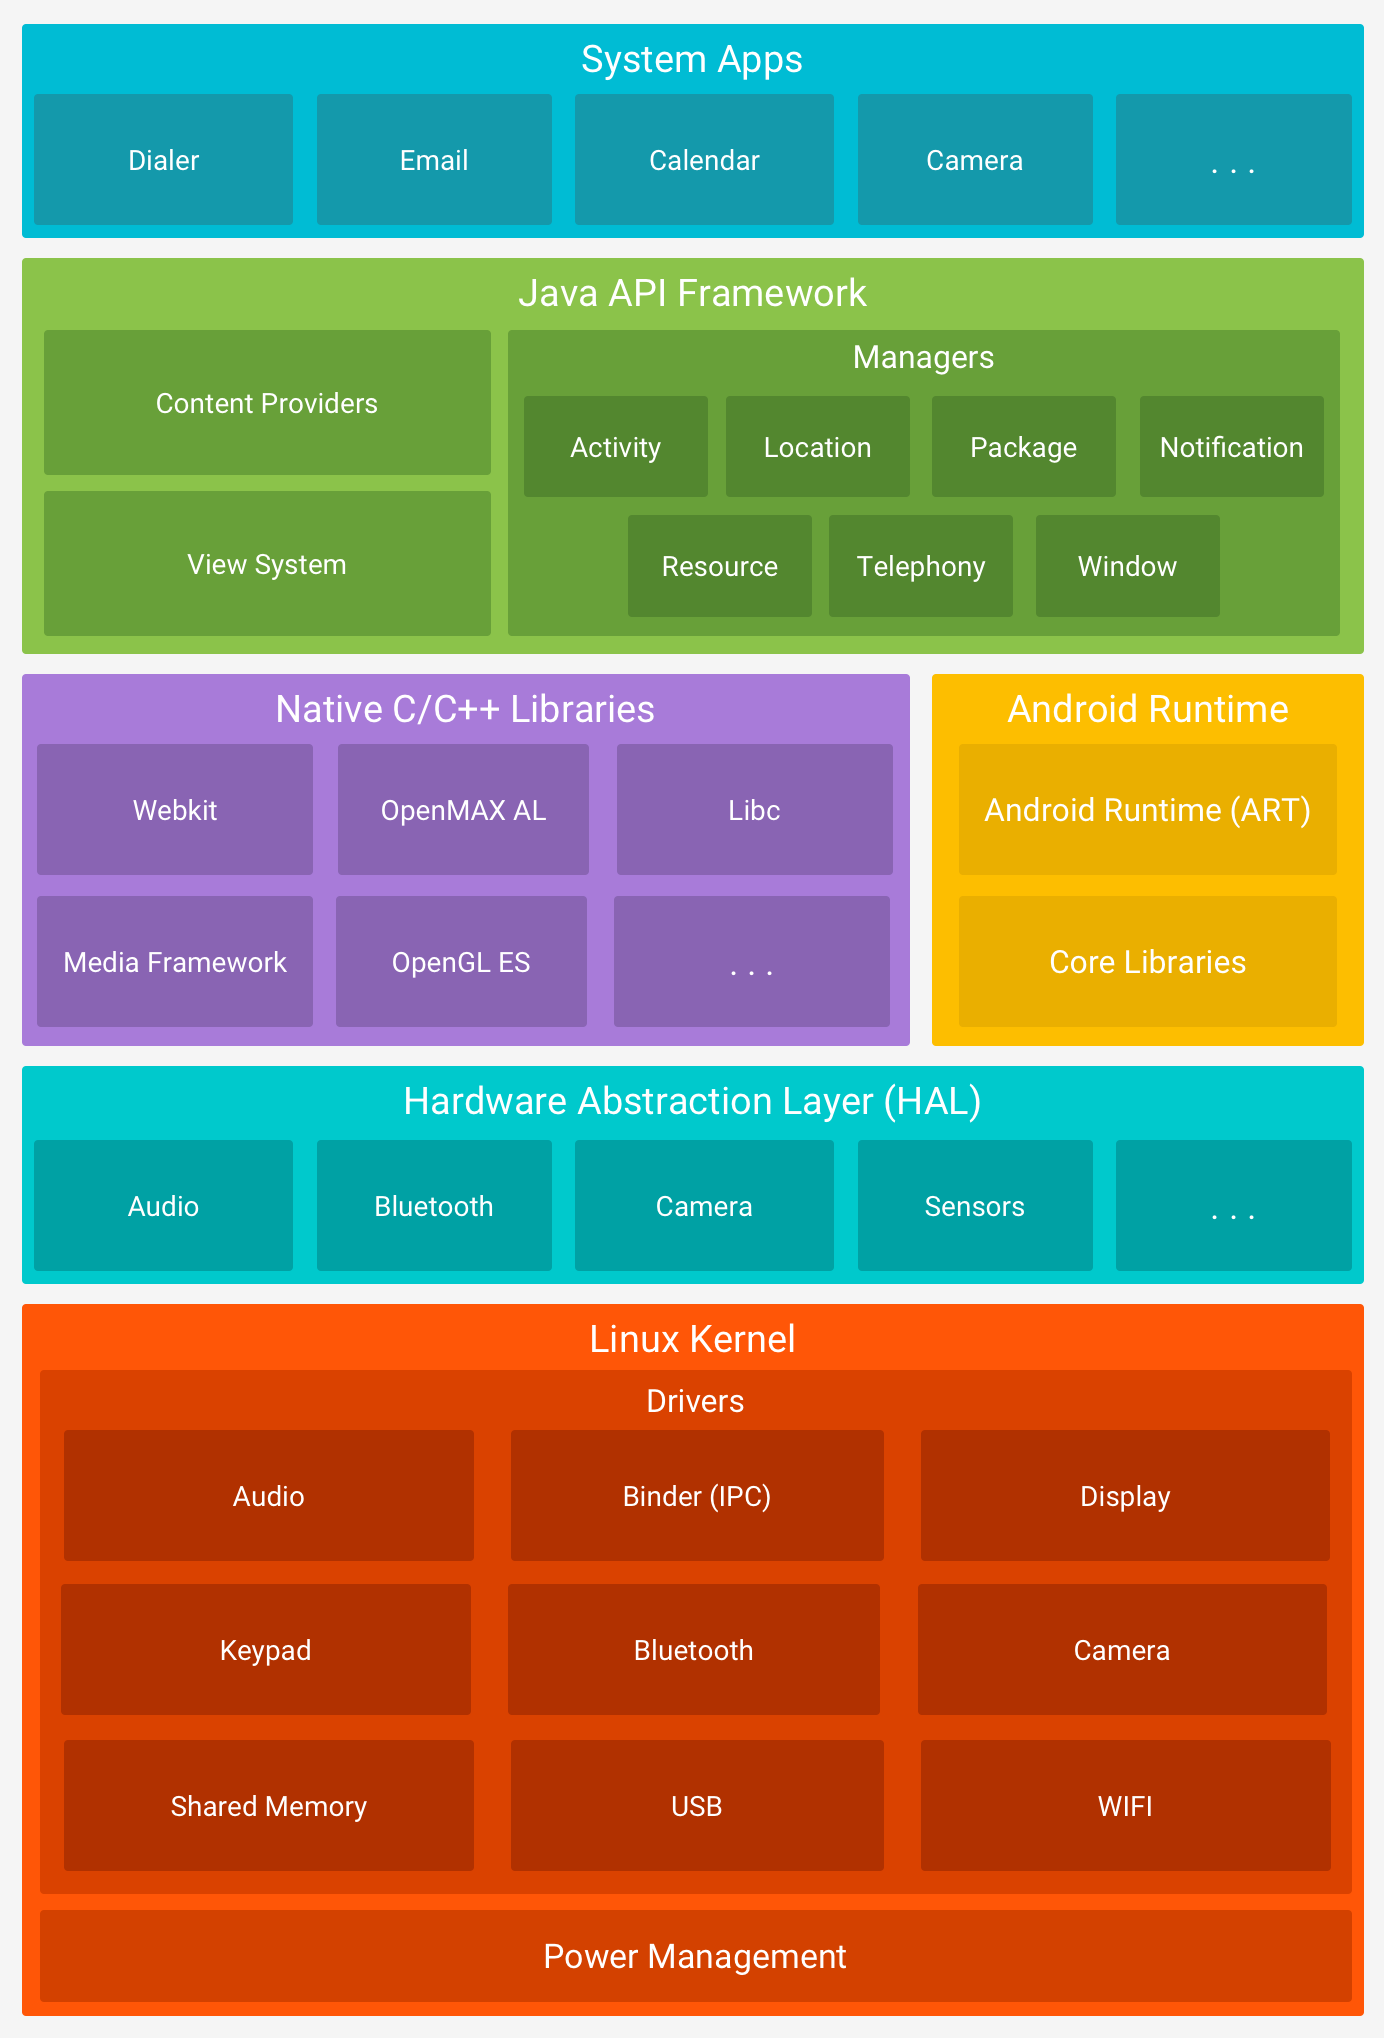
\includegraphics[scale=0.1]{android-stack_2x.png}

\end{multicols}

\subsection{Kernel}

\begin{multicols}{2}

\subsubsection{Modifiactions}

\begin{flushleft}
  Modifications made by android to linux OS
\end{flushleft}
\begin{itemize}
  \item wakelocks – keep the phone awake
  \item binder – interprocess communication
  \item ashmem – shared memory
  \item oom – kills processes when memory is low
  \item alarm manager – wakes up the phone when necessary
\end{itemize}

\vfill\null

\subsection{Hardware support}
\begin{itemize}
  \item Bluetooth - BlueZ
  \item GPS – Manufacturer provided libgps
  \item Wifi – \texttt{wpa-supplicant}
  \item Display – Standard framebuffer driver
  \item Keyboard – Standard input event
  \item Lights – Manufacturer provided liblights.so
  \item Audio – Manufacturer provided libaudio.so
  \item Camera – Manufacturer provided libcamera.so
  \item Power Management – “wakelocks” kernel patch
  \item Sensors – Manufacturer provided libsensors.so
  \item Radio – Manufacturer provided libril.so
\end{itemize}

\end{multicols}

\subsection{Security}

Applications are sandboxed
\begin{itemize}
 \item A security mechanism for separating running applications and data
 \item This allows applications run in a different context, so if one app crashed, others can stay uneffected
 \item On Android, each app runs as its own \textbf{user}, which guarantees that different users are unable to interfere with each other, access each other’s files and so on. Root can access the entire system
 \item Own process, own VM, own UID/AID for different app
\end{itemize}

\newpage

\begin{description}
	\item[placeholder] \hfill \\
\end{description}
\end{document}
